\section{과제풀이}
\subsection{과제 1}
\begin{figure}[!hbpt]
\centering
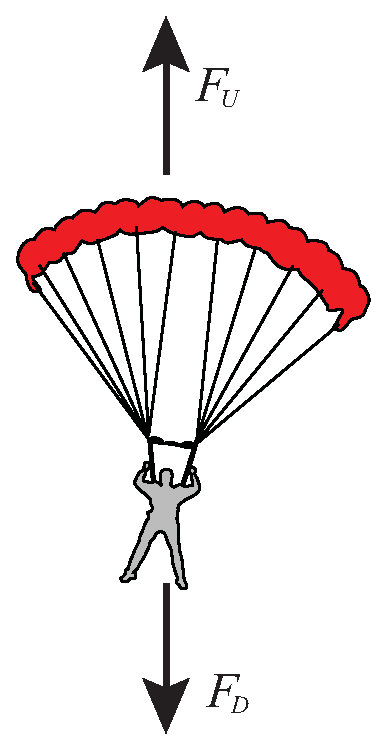
\includegraphics[keepaspectratio=true,width=0.2\linewidth]{figs/parachute.eps}
%\caption{낙하산병에 작용하는 힘에 대한 개략도. $F_D$는 중력에 의해 아래로 작용하는 힘이고, $F_U$는 공기의 저항에 의하여 위로 작용하는 힘이다.}
\label{fig:b-2}
\end{figure}
\subsubsection{낙하산병의 초기속도 $v(0)$가 $0$이 아닌 경우, $v(0)$ 상수를 도입하여 정밀해를 구하라}
\begin{equation}
\frac{dv}{dt}=g-\frac{c}{m}v
\label{eq:b-7}
\end{equation}
\rule{\textwidth}{0.1pt}
\framebox[1.1\width]{풀이} 강의노트에서 해석해 풀이과정과 유사하게 변수분리방법을 사용하면
\begin{equation}
\frac{m}{mg-cv}dv=1\cdot dt
\label{eq:b-8}
\end{equation}
양변을 적분하면 식(\ref{eq:b-8})은 시각 $T$에서 다음과 같이 변형할 수 있다.
\begin{equation}
\int_{v(0)}^{v(T)}\frac{m}{mg-cv}dv=\int_{0}^{T}1\cdot dt
\label{eq:b-9}
\end{equation}
초기속도가 $0$이 아니기 때문에 즉, $t=0$일때, $v(0)$로 놓고, $mg-cv$를 시간의 종속변수$X$로 치환하면,
\begin{eqnarray}
mg-cv=X\\
\frac{dX}{dv}=-c\\
dv=-\frac{1}{c}dx
\end{eqnarray}
치환변수 $X$의 초기값과 $T$에서의 값은 각각, $X(0)=mg-cv(0)$ 그리고 $X(T)=mg-cv(T)$가 된다. 다시 식(\ref{eq:b-9})에 대입하면,
\begin{equation}
-\frac{m}{c}\int_{X(0)}^{X(T)}\frac{1}{X}dv=\int_{0}^{T}1\cdot dt
\label{eq:b-10}
\end{equation}
식(\ref{eq:b-10})을 계산하면,
\begin{equation}
-\frac{m}{c}\ln X\arrowvert_{X(0)}^{X(T)}=T
\end{equation}
치환된 변수를 환원하면서 전개하면,
\begin{equation}
-\frac{m}{c}\left[\ln\left\{mg-cv(T)\right\}-\ln\left\{mg-cv(0)\right\}\right] = T
\end{equation}
정리하면
\begin{equation}
\ln\left(\frac{mg-cv(T)}{mg-cv(0)}\right) = -\frac{c}{m}T
\end{equation}
양변에 $\ln$을 취하면,
\begin{equation}
e^{-(c/m)T}=\frac{mg-cv(T)}{mg-cv(0)}
\end{equation}
함수$v(T)$를 구하기위해 정리하면
\begin{align}
\left\{mg-cv(0)\right\}e^{-(c/m)T}&=mg-cv(T)\\
v(T)&=\frac{mg}{c}-\frac{\left\{mg-cv(0)\right\}}{c}e^{-(c/m)T}
\end{align}
결국 시각 $T$에서 엄밀해는 식(\ref{eq:b-11})과 같이 계산된다.
\begin{equation}
v(T)=\frac{mg}{c}\left(1-e^{-(c/m)T}\right)+v(0)e^{-(c/m)T}
\label{eq:b-11}
\end{equation}
\rule{\textwidth}{0.1pt}
\subsubsection{낙하하는 낙하산병에게 작용하는 힘을 계산하는 과정에서, 식(\ref{eq:b-7})로 주어진 선형관계식 대신, 다음과 같은 2차식을 사용하여 정밀해 혹은 수치해를 구하여라}

\begin{displaymath}
F_{U}=-c'v^2
\end{displaymath}
단, $c'$은 2차항력계수($kg/m$)이며, 수치해를 구할땐, 10초후의 낙하산병의 속도를 구하라. 여기서, 낙하산병의 질량은 68.1kg이고 2차항력계수는 $0.232kg/m$이다.\\
\rule{\textwidth}{0.1pt}
\framebox[1.1\width]{풀이(정확해)}\\
같은 방식으로 식(\ref{eq:b-7})을 속도의 제곱항으로 변형하면,
\begin{align}
\frac{dv}{dt}&=g-\frac{c'}{m}v^2\\
&=\frac{mg-c'v^2}{m}
\end{align}
같은 방식으로 변수분리 방식을 사용하기 위해 식을 변형하면,
\begin{equation}
\frac{m}{mg-c'v^2}dv=1\cdot dt
\end{equation}
양변의 시간 $t=0$에서 $t=T$까지 정적분을 취하면,
\begin{equation}
\int_{v(0)}^{v(T)}\frac{m}{mg-c'v^2}dv=\int_{0}^{T}dt
\end{equation}
다음 식(\ref{eq:b-19})과 같은 적분공식을 적용하기 위하여 식을 변형하고
\begin{equation}
\int\frac{1}{a^2-x^2}dx=\frac{1}{a}\tanh^{-1}\frac{x}{a}+C
\label{eq:b-19}
\end{equation}
적분식에서 발생하는 $\sqrt{c'}v$항을 $X$로 치환하면
\begin{align}
m\int_{v(0)}^{v(T)}\frac{1}{(\sqrt{mg})^2-(\sqrt{c'}v)^2}&=\int_{0}^{T}dt\\
\frac{m}{\sqrt{c'}}\int_{X(0)}^{X(T)}\frac{1}{\sqrt{mg}^2-X^2}dX&=\int_{0}^{T}dt
\end{align}
여기서, 치환변수 $X=\sqrt{c'}v$는, $dX/dv=\sqrt{c'}$, $dv=(1/\sqrt{c'})dX$로 변형되고, 적분구간은 $X(0)=v(0)=0$, $X(T)=\sqrt{c'}v(T)$로 변형된다. 정적분을 풀고 이항하여 $v(T)$로 정리하면,
\begin{align}
\frac{m}{\sqrt{c'}}\left[\frac{1}{\sqrt{mg}}\tanh^{-1}\frac{X}{\sqrt{mg}}\right]_{X(0)}^{X(T)}&=T\\
\frac{m}{\sqrt{mgc'}}\tanh^{-1}\left(\sqrt{\frac{c'}{mg}}v(T)\right)&=T\\
\tanh^{-1}\left(\sqrt{\frac{c'}{mg}}v(T)\right)&=\frac{\sqrt{gc'}{m}}T\\
\sqrt{\frac{c'}{mg}}v(T)&=\tanh\left(\sqrt{\frac{gc'}{m}}T\right)\\
\therefore v(t)=\sqrt{\frac{mg}{c'}}\tanh\left(\sqrt{\frac{gc'}{m}}T\right)
\end{align}
\framebox[1.1\width]{풀이(수치해)}\\
부록1장에 수록된 MATLAB Code에서 \texttt{v(kk)}를 \texttt{v(kk)\^{}2}로 수정한다.
\lstinputlisting[language=Matlab, label=lst:report1-2, caption=2번문제 수치해]{MATLAB/report1s2.m}

\rule{\textwidth}{0.1pt}

\subsubsection{테일러급수(Taylor series)를 증명하라.}
\begin{equation*}
f(x)=\sum_{n=0}^{\infty}\frac{f^{(n)}(a)}{n!}(x-a)^{n}
\end{equation*}
\rule{\textwidth}{0.1pt}
\framebox[1.1\width]{풀이}
Taylor급수를 증명하기 위해서는 미적분학 제1기본정리와 제2기본정리를 알아야한다.\\
\begin{tabular}[c]{|p{\textwidth}|}
\hline
\begin{theorem}[미적분학 제1기본정리]
함수 $f$가 폐구간 $[a,b]$에서 적분가능할 때, 함수 $F$를 $F(x)=\int_{a}^{x}f(t)dt$라 하면, 이때 다음이 성립한다.
$f$가 $[a,b]$상의 점 $c$에서 연속이면, $F$는 $[a,b]$에서 미분가능하고, $F'(c) = f(c)$이다. 즉,
\begin{equation}
F'(x)=\frac{d}{dx}\int_{a}^{x}f(t)dt=f(x)
\end{equation}
\end{theorem}
\\\hline
\end{tabular}

\begin{proof1}
$S(x)=\int_{a}^{x}f(t)dt$함수 $f(t)$에 대해 $[a,b]$에서 연속이고, $(a,b)$에서 미분가능하므로 함수 $S(x)$도 $[a,b]$에서 연속하고 $(a,b)$에서 미분가능하다.
최대최소 정리에 의해 $h>0$ 일 때 $[x, x+h]$에서 $f(t)$는 최대값 $M$과 최소값 $m$을 가진다.
여기서 $mh<S(x+h)-S(x)<Mh$이므로 
\begin{equation*}
\lim_{h\rightarrow0}m\leq\lim_{h\rightarrow0}\frac{S(x+h)-S(x)}{h}\leq\lim_{h\rightarrow0}M
\end{equation*}
이다, 즉 압착정리에 의해 $\lim_{h\rightarrow0}m=\lim_{h\rightarrow0}M=f(x)=S'(x)$이 되므로, $S'(x)=f(x)$가 성립한다.
\end{proof1}
\begin{tabular}[c]{|p{\textwidth}|}
\hline
\begin{theorem}[미적분학 제2기본정리]
$f$가 폐구간 $[a,b]$에서 적분가능한 함수이고, 함수 $F$를 $f$의 임의의 역도함수라 하면, 다음식
\begin{equation}
\int_{a}^{b}f(t)dt=F(b)-F(a)
\end{equation}
이 성립한다. 즉, 정적분은 임의의 역도함수의 차로 계산할 수 있다.
\end{theorem}
\\\hline
\end{tabular}

\begin{proof1}
미적분학 제1기본정리에서 $S(x)=F(x)+C$(단, $C$는 적분상수)에서, $S(x)=\int_{a}^{x}f(t)dt$로 정의되었으므로,
\begin{equation}
S(a)=F(a)+C=0
\end{equation}
위 식에서 $C=-F(a)$, $S(x)=\int_{a}^{x}f(t)dt=F(x)-F(a)$이다. 따라서,
\begin{equation}
\int_{a}^{b}f(x)dx=F(b)-F(a)
\end{equation}
이 성립한다.
\end{proof1}

\begin{proof1}[Taylor series]
미적분학 제2기본정리로부터,
\begin{equation}
\int_{a}^{x}f'(t)dt=f(x)-f(a)
\label{eq:t1}
\end{equation}
위의 식(\ref{eq:t1})을 부분적분을 하기 위해 다음 식(\ref{eq:t2})로 변형하자
\begin{equation}\label{eq:t2}
\int_{a}^{x}f'(t)dt=\int_{a}^{x}(-1)\left\{-f'(t)\right\}dt
\end{equation}
$f(t)$는 무한번 미분가능하면 부분적분을 무한번 수행할 수 있으므로, $-1$을 적분할 함수, $-f'(t)$를 미분할 함수로 두고, 부분적분을 수행하면\footnote{단, 여기서 $-1$을 계속 적분할 때 $-1$의 한 부정적분을 구해서 써주면 되는데, 적분변수 $t$와 관계없는 값$x$를 상수취급하여 $x-t$를 부정적분으로서 구했다.},
\begin{equation}\label{eq:t3}
\int_{a}^{x}(-1)\left\{-f'(t)\right\}dt =\left[-(x-t)f'(t)-\frac{(x-t)^2}{2}f''(t)-\frac{(x-t)^3}{6}f'''(t)-\cdots\right]_{a}^{x}
\end{equation}
이제 식(\ref{eq:t3})을 풀게되면,
\begin{equation}\label{eq:t4}
\begin{split}
\left[-(x-t)f'(t)-\frac{(x-t)^2}{2}f''(t)-\frac{(x-a)^3}{6}f'''(t)-\cdots\right] &= (x-a)f'(a)+\frac{(x-a)^2}{2!}f'''(a)+\frac{(x-a)^3}{3!}f'''(a)+\cdots\\
&=f(x)-f(a)
\end{split}
\end{equation}
그러므로, 무한번 미분가능한 함수 $f(x)$에 대하여
\begin{align}
f(x)&=f(a)+(x-a)f'(a)+\frac{(x-a)^2}{2!}f''(a)+\frac{(x-a)^3}{3!}f'''(a)+\cdots\\
&=\sum_{n=0}^{\infty}\frac{f^{(n)}(a)}{n!}(x-a)^{n}
\end{align}
\end{proof1}
\rule{\textwidth}{0.1pt}

%\section{공학 수치해석 과제풀이2}
%\subsection{$\cos x$의 Maclaurin 급수는 다음과 같이 주어진다.}
%\begin{equation}
%\begin{split}
%\cos x&=\sum_{n=0}^{\infty}\frac{(-1)^n}{(2n)!}x^{2n}\\
%&=1-\frac{x^2}{2!}+\frac{x^4}{4!}-\frac{x^6}{6!}+\frac{x^8}{8!}-\cdots
%\end{split}
%\end{equation}
%가장 간단한 형태인 $\cos x =1$로부터 시작하여 항들을 추가해 가면서 $\cos(\pi/3)$의 값을 구하라. 각각의 항이 추가될 때마다, 절단오차(상대오차)를 계산하라.\\
%
%
%2. $x\in \Re$에 대하여 $|x|>1$의 개구간 미분이 가능한 다음 함수$f(x)$의 Taylor 급수를 전개하고, $x=3$에서 5차 근사값을 구하고, 절단오차 $E_{t}$를 각각의 차수에 대하여 표시하라.
%\begin{displaymath}
%f(x)=\frac{x}{x-1}
%\end{displaymath}
%3. 다음 함수 $f(x)=\ln(\cos x), x\in (-\pi/2,\pi/2)$를 7차이상의 다항식으로 전개하라\\
%
%참고 Maclaurin 급수
%\begin{eqnarray*}
%\ln(1-x)&=&-\sum_{n=1}^{\infty}\frac{x^n}{n}, (|x|\leq 1, x\neq 1)\\
%\ln(1+x)&=&\sum_{n=1}^{\infty}(-1)^{n+1}\frac{x^n}{n}, (|x|\leq 1, x\neq -1)
%\end{eqnarray*}
%4. 정확도(accuracy)와 정밀도(precision)에 대하여 조사하라\footnote{\url{http://en.wikipedia.org/wiki/Accuracy_and_precision}} 그리고 각 전공영역에 맞추어  특정한 공학적 이슈를 예를들어 불확실성(uncertainty)에 대하여 자신의 생각을 쓰시오.
